\model{Yahtzee Dice}

Creating an array of objects is typically a 3-step process:

\begin{center}
%TODO where did this image come from? Ralph Grove?
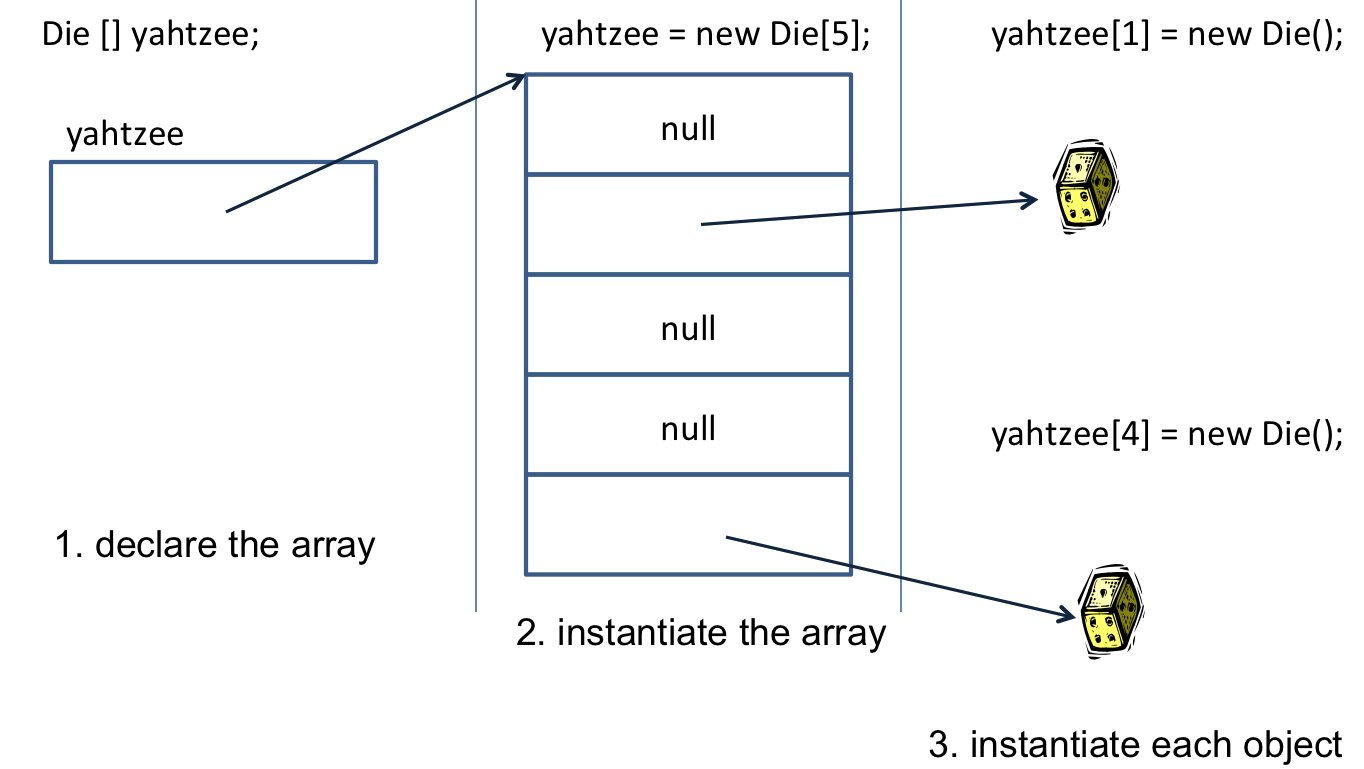
\includegraphics[width=5.5in]{yahtzee-array.png}
\end{center}


\quest{15 min}


\Q What is the type of the local variable \java{yahtzee}?
What is its initial value? (Hint: it's not \java{null}.)

\begin{answer}
It's an array of \java{Die} objects. Until it's assigned for the first time, it's uninitialized (meaning you that can't read its value).
\end{answer}


\Q When you create an array (e.g., ~\java{new Die[5]}) what is the initial value of each element?

\begin{answer}
The initial values are automatically set to null (for reference types). For arrays of integers, it's 0; for doubles, it's 0.0; for booleans, it's {\tt false}; for characters, it's the unicode character \chr{\textbackslash u0000}.
\end{answer}


\Q When you construct a new object (e.g., ~\java{new Die()}) what are the initial values of its attributes (e.g., ~\java{this.face})?

\begin{answer}
All attributes are initialized to the value of ``zero'' for that data type.
So references are {\tt null}, integers are 0, doubles are 0.0, and so forth.
\end{answer}


\Q Describe in your own words what the following statement does. Be sure to explain how the random part works.

\begin{center}
\java{yahtzee[(int) (Math.random() * yahtzee.length)] = null;}
\end{center}

\begin{answer}
\java{Math.random()} returns a value in the range [0, 1).
Multiplying that value by \java{yahtzee.length} and then casting it to an integer gives a value in the range 0..5 inclusive.
So this statement randomly sets of the dice references to {\tt null}.
\end{answer}


\Q \label{fordie} What is the result of running the loop below?
What is the purpose of the nested if-statement?

\begin{javalst}
for (int i = 0; i < yahtzee.length; i++) {
    if (yahtzee[i] != null) {
        yahtzee[i].roll();
    }
}
\end{javalst}
\vspace{-1ex}

\begin{answer}
This loop rolls the dice in the array.
Because some of the dice are {\tt null}, the if-statement prevents {\tt NullPointerException}.
\end{answer}


\Q The enhanced for loop allows you to iterate the elements of an array.
Another name for this structure is the ``for each'' loop.
Rewrite the following example using a standard for loop.

\vspace{1ex}
\begin{javalst}
String[] days = {"Sun", "Mon", "Tue", "Wed", "Thu", "Fri", "Sat"};
for (String day : days) {
    System.out.println(day + " is a great day!");
}
\end{javalst}
\vspace{-1em}

\begin{answer}[5em]
\begin{javaans}
for (int i = 0; i < days.length; i++) {
    System.out.println(days[i] + " is a great day!");
}
\end{javaans}
\end{answer}


\Q In contrast to enhanced for loops, what does a standard for loop typically iterate?
Why would it be misleading to name the enhanced for loop variable \java{i} instead of \java{day}?

\begin{answer}
Standard for loops typically iterate indexes; that's why the variable is almost always named \java{i}.
\end{answer}


\Q Rewrite the loop in \ref{fordie} using an enhanced for loop.
Use an appropriate variable name for the \java{Die} object (i.e., not \java{i}).

\vspace{-1ex}
\begin{answer}[7em]
\begin{javaans}
for (Die die : yahtzee) {
    if (die != null) {
        die.roll();
    }
}
\end{javaans}
\end{answer}
